\documentclass[11pt,a4paper]{report}
\usepackage[textwidth=37em,vmargin=30mm]{geometry}
\usepackage{calc,xunicode,amsmath,amssymb,paralist,enumitem,tabu,booktabs,datetime2,xeCJK,xeCJKfntef,listings}
\usepackage{tocloft,fancyhdr,tcolorbox,xcolor,graphicx,eso-pic,xltxtra,xelatexemoji}

\newcommand{\envyear}[0]{2025}
\newcommand{\envdatestr}[0]{2025-06-16}
\newcommand{\envfinaldir}[0]{webdb/2025/20250616/final}

\usepackage[hidelinks]{hyperref}
\hypersetup{
    colorlinks=false,
    pdfpagemode=FullScreen,
    pdftitle={Web Digest - \envdatestr}
}

\setlength{\cftbeforechapskip}{10pt}
\renewcommand{\cftchapfont}{\rmfamily\bfseries\large\raggedright}
\setlength{\cftbeforesecskip}{2pt}
\renewcommand{\cftsecfont}{\sffamily\small\raggedright}

\setdefaultleftmargin{2em}{2em}{1em}{1em}{1em}{1em}

\usepackage{xeCJK,xeCJKfntef}
\xeCJKsetup{PunctStyle=plain,RubberPunctSkip=false,CJKglue=\strut\hskip 0pt plus 0.1em minus 0.05em,CJKecglue=\strut\hskip 0.22em plus 0.2em}
\XeTeXlinebreaklocale "zh"
\XeTeXlinebreakskip = 0pt


\setmainfont{Brygada 1918}
\setromanfont{Brygada 1918}
\setsansfont{IBM Plex Sans}
\setmonofont{JetBrains Mono NL}
\setCJKmainfont{Noto Serif CJK SC}
\setCJKromanfont{Noto Serif CJK SC}
\setCJKsansfont{Noto Sans CJK SC}
\setCJKmonofont{Noto Sans CJK SC}

\setlength{\parindent}{0pt}
\setlength{\parskip}{8pt}
\linespread{1.15}

\lstset{
	basicstyle=\ttfamily\footnotesize,
	numbersep=5pt,
	backgroundcolor=\color{black!5},
	showspaces=false,
	showstringspaces=false,
	showtabs=false,
	tabsize=2,
	captionpos=b,
	breaklines=true,
	breakatwhitespace=true,
	breakautoindent=true,
	linewidth=\textwidth
}






\newcommand{\coverpic}[2]{
    % argv: itemurl, authorname
    Cover photo by #2~~(\href{#1}{#1})
}
\newcommand{\makeheader}[0]{
    \begin{titlepage}
        % \newgeometry{hmargin=15mm,tmargin=21mm,bmargin=12mm}
        \begin{center}
            
            \rmfamily\scshape
            \fontspec{BaskervilleF}
            \fontspec{Old Standard}
            \fontsize{59pt}{70pt}\selectfont
            WEB\hfill DIGEST
            
            \vfill
            % \vskip 30pt
            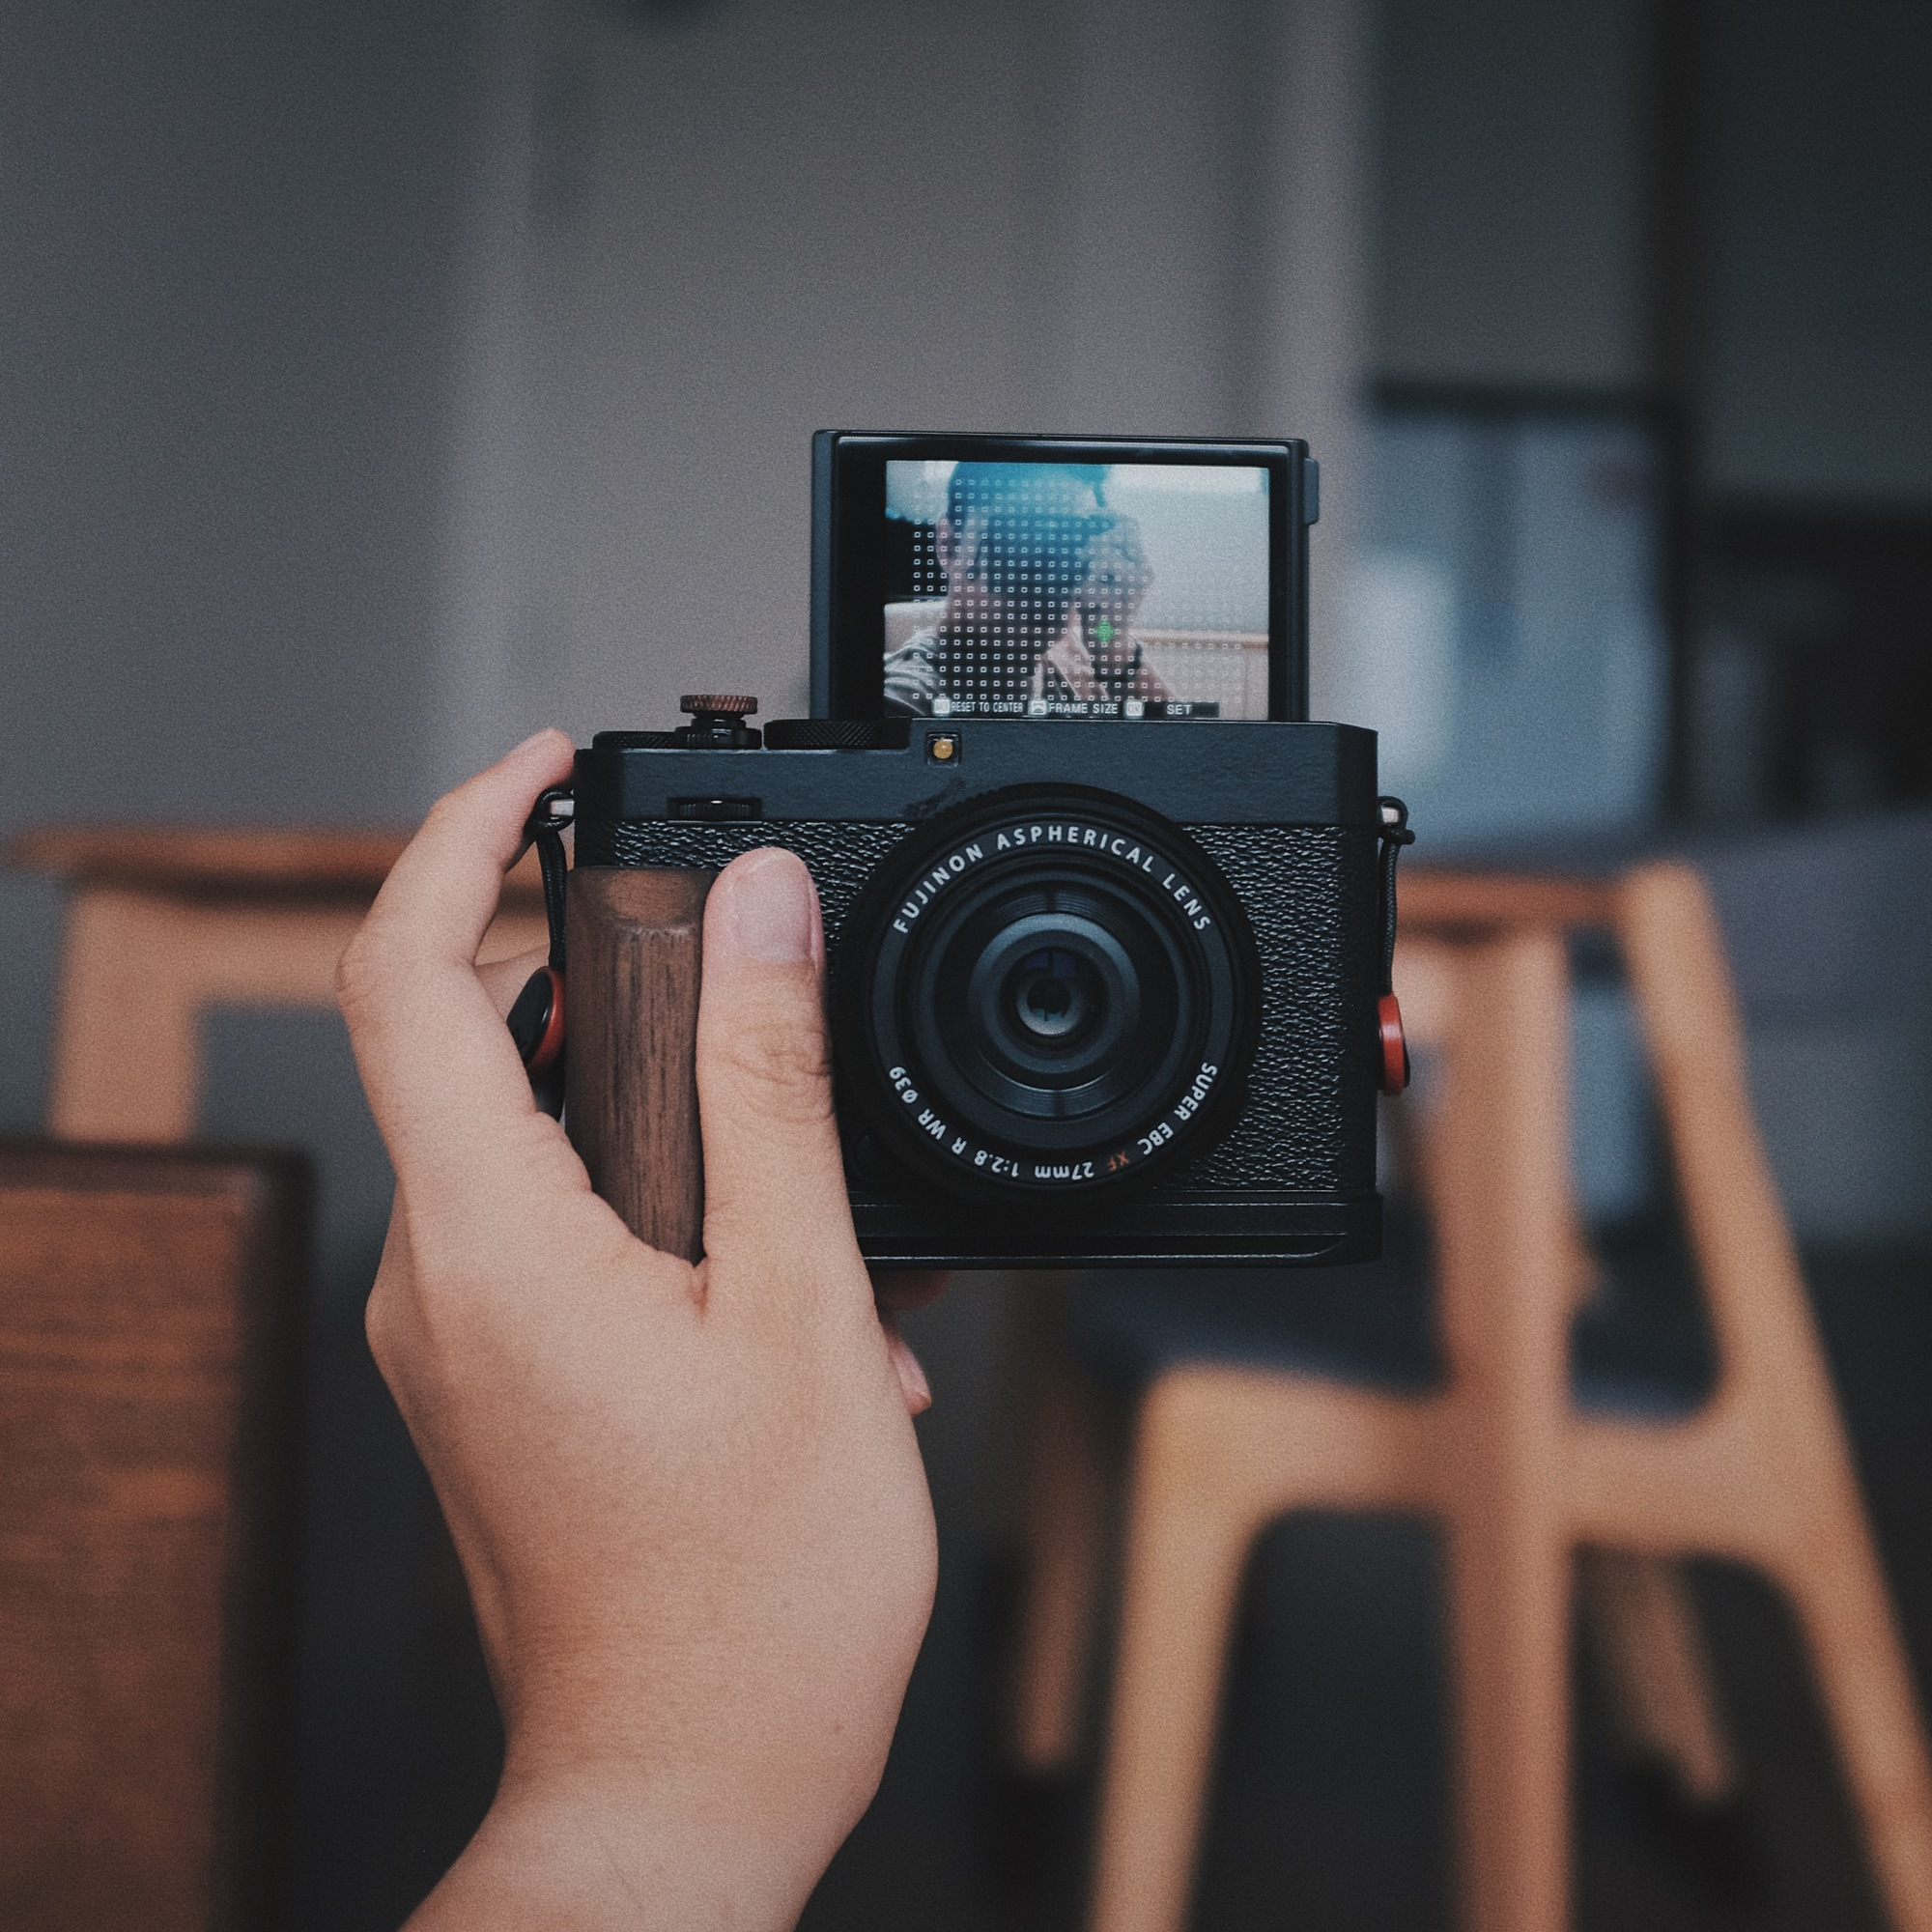
\includegraphics[width=\linewidth]{\envfinaldir/coverpic-prod.jpg}\par
            % \vskip 30pt
            \vfill

            \normalsize\rmfamily\scshape
            \copyright{} The Web Digest Project \hfill\large \envdatestr
        \end{center}
    \end{titlepage}
    % \restoregeometry
}
\newcommand{\simplehref}[1]{%
    \textcolor{blue!80!green}{\href{#1}{#1}}%
}
\renewcommand{\contentsname}{\center\Huge\sffamily\bfseries Contents\par\vskip 20pt}
\newcounter{ipartcounter}
\setcounter{ipartcounter}{0}
\newcommand{\ipart}[1]{
    % \vskip 20pt
    \clearpage
    \stepcounter{ipartcounter}
    \phantomsection
    \addcontentsline{toc}{chapter}{#1}
    % \begin{center}
    %     \Huge
    %     \sffamily\bfseries
    %     #1
    % \end{center}
    % \vskip 20pt plus 7pt
}
\newcounter{ichaptercounter}
\setcounter{ichaptercounter}{0}
\newcommand{\ichapter}[1]{
    % \vskip 20pt
    \clearpage
    \stepcounter{ichaptercounter}
    \phantomsection
    \addcontentsline{toc}{section}{\numberline{\arabic{ichaptercounter}}#1}
    \begin{center}
        \Huge
        \sffamily\bfseries
        #1
    \end{center}
    \vskip 20pt plus 7pt
}
\newcommand{\entrytitlefont}[1]{\subsection*{\raggedright\Large\sffamily\bfseries#1}}
\newcommand{\entryitemGeneric}[2]{
    % argv: title, url
    \parbox{\linewidth}{
        \entrytitlefont{#1}\par\vskip 5pt
        \footnotesize\ttfamily\mdseries
        \simplehref{#2}
    }\vskip 11pt plus 11pt minus 1pt
}
\newcommand{\entryitemGithub}[3]{
    % argv: title, url, desc
    \parbox{\linewidth}{
        \entrytitlefont{#1}\par\vskip 5pt
        \footnotesize\ttfamily\mdseries
        \simplehref{#2}\par\vskip 5pt
        \small\rmfamily\mdseries#3
    }\vskip 11pt plus 11pt minus 1pt
}
\newcommand{\entryitemAp}[3]{
    % argv: title, url, desc
    \parbox{\linewidth}{
        \entrytitlefont{#1}\par\vskip 5pt
        \footnotesize\ttfamily\mdseries
        \simplehref{#2}\par\vskip 5pt
        \small\rmfamily\mdseries#3
    }\vskip 11pt plus 11pt minus 1pt
}
\newcommand{\entryitemHackernews}[3]{
    % argv: title, hnurl, rawurl
    % \parbox{\linewidth}{
    %     \entrytitlefont{#1}\par\vskip 5pt
    %     \footnotesize\ttfamily\mdseries
    %     \simplehref{#3}\par
    %     \textcolor{black!50}{\href{#2}{#2}}
    % }\vskip 11pt plus 11pt minus 1pt
    \begin{minipage}{\linewidth}
            \entrytitlefont{#1}\par\vskip 5pt
            \footnotesize\ttfamily\mdseries
            \simplehref{#3}\par
            \textcolor{black!50}{\href{#2}{#2}}
    \end{minipage}\par\vskip 11pt plus 11pt minus 1pt
}







\begin{document}

\makeheader

\tableofcontents\clearpage




\ipart{Developers}
\ichapter{Hacker News}
\entryitemTwoLinks{Social anxiety disorder-associated gut microbiota increases social fear}{https://news.ycombinator.com/item?id=44283095}{https://www.pnas.org/doi/abs/10.1073/pnas.2308706120}

\entryitemTwoLinks{GNOME and Red Hat Linux eleven years ago (2009)}{https://news.ycombinator.com/item?id=44283047}{https://linuxgazette.net/165/laycock.html}

\entryitemTwoLinks{Modifying an HDMI dummy plug's EDID using a Raspberry Pi}{https://news.ycombinator.com/item?id=44282998}{https://www.downtowndougbrown.com/2025/06/modifying-an-hdmi-dummy-plugs-edid-using-a-raspberry-pi/}

\entryitemTwoLinks{Journalists Wary of Travelling to US Due to Palantir Surveillance}{https://news.ycombinator.com/item?id=44282754}{https://bsky.app/profile/alistairkitchen.bsky.social/post/3lrjsdecc5c2x}

\entryitemTwoLinks{Nvidia CEO criticizes Anthropic boss over his statements on AI}{https://news.ycombinator.com/item?id=44282657}{https://www.tomshardware.com/tech-industry/artificial-intelligence/nvidia-ceo-slams-anthropic-chief-over-claims-of-job-eliminations-says-many-jobs-are-going-to-be-created}

\entryitemTwoLinks{Why SSL was renamed to TLS in late 90s (2014)}{https://news.ycombinator.com/item?id=44282378}{https://tim.dierks.org/2014/05/security-standards-and-name-changes-in.html}

\entryitemTwoLinks{Canyon.mid}{https://news.ycombinator.com/item?id=44282177}{https://canyonmid.com/}

\entryitemTwoLinks{Childhood leukemia: how a deadly cancer became treatable}{https://news.ycombinator.com/item?id=44282143}{https://ourworldindata.org/childhood-leukemia-treatment-history}

\entryitemTwoLinks{How to modify Starlink Mini to run without the built-in WiFi router}{https://news.ycombinator.com/item?id=44282017}{https://olegkutkov.me/2025/06/15/how-to-modify-starlink-mini-to-run-without-the-built-in-wifi-router/}

\entryitemTwoLinks{Datalog in Rust}{https://news.ycombinator.com/item?id=44281727}{https://github.com/frankmcsherry/blog/blob/master/posts/2025-06-03.md}

\entryitemTwoLinks{Foundations of Computer Vision}{https://news.ycombinator.com/item?id=44281506}{https://visionbook.mit.edu}

\entryitemTwoLinks{The Art of Lisp and Writing (2003)}{https://news.ycombinator.com/item?id=44281016}{https://www.dreamsongs.com/ArtOfLisp.html}

\entryitemTwoLinks{Q-learning is not yet scalable}{https://news.ycombinator.com/item?id=44279850}{https://seohong.me/blog/q-learning-is-not-yet-scalable/}

\entryitemTwoLinks{Infinite Grid of Resistors}{https://news.ycombinator.com/item?id=44279181}{https://www.mathpages.com/home/kmath668/kmath668.htm}

\entryitemTwoLinks{AMD's AI Future Is Rack Scale 'Helios'}{https://news.ycombinator.com/item?id=44278746}{https://morethanmoore.substack.com/p/amds-ai-future-is-rack-scale-helios}

\entryitemTwoLinks{Seven replies to the viral Apple reasoning paper and why they fall short}{https://news.ycombinator.com/item?id=44278403}{https://garymarcus.substack.com/p/seven-replies-to-the-viral-apple}

\entryitemTwoLinks{Waymo's market share in San Francisco exceeds Lyft's}{https://news.ycombinator.com/item?id=44277355}{https://underscoresf.com/in-san-francisco-waymo-has-now-bested-lyft-uber-is-next/}

\entryitemTwoLinks{SSHTron: A multiplayer lightcycle game that runs through SSH}{https://news.ycombinator.com/item?id=44277245}{https://github.com/zachlatta/sshtron}

\entryitemTwoLinks{Inside the Apollo ``8-Ball'' FDAI (Flight Director / Attitude Indicator)}{https://news.ycombinator.com/item?id=44277051}{https://www.righto.com/2025/06/inside-apollo-fdai.html}

\entryitemTwoLinks{I have reimplemented Stable Diffusion 3.5 from scratch in pure PyTorch}{https://news.ycombinator.com/item?id=44276476}{https://github.com/yousef-rafat/miniDiffusion}\ichapter{Dribbble}
\entryitemGeneric{\hskip 0pt{}Aquasan}{https://dribbble.com/shots/26100535-Aquasan}

\entryitemGeneric{\hskip 0pt{}Eagle}{https://dribbble.com/shots/26099428-Eagle}

\entryitemGeneric{\hskip 0pt{}Mnp Technologies - Logo Design}{https://dribbble.com/shots/26092034-Mnp-Technologies-Logo-Design}

\entryitemGeneric{\hskip 0pt{}Singular Logo Concept (Unused)}{https://dribbble.com/shots/26091755-Singular-Logo-Concept-Unused}

\entryitemGeneric{\hskip 0pt{}Cre8tera // Website}{https://dribbble.com/shots/26091009-Cre8tera-Website}

\entryitemGeneric{\hskip 0pt{}Cool Pool Logo Design - Letter C Monogram}{https://dribbble.com/shots/26091401-Cool-Pool-Logo-Design-Letter-C-Monogram}

\entryitemGeneric{\hskip 0pt{}Gorilla + Bar Chart Logo}{https://dribbble.com/shots/26092670-Gorilla-Bar-Chart-Logo}

\entryitemGeneric{\hskip 0pt{}zeero logo design}{https://dribbble.com/shots/26087342-zeero-logo-design}

\entryitemGeneric{\hskip 0pt{}Create email inbox composition}{https://dribbble.com/shots/26083118-Create-email-inbox-composition}

\entryitemGeneric{\hskip 0pt{}Shori Brand}{https://dribbble.com/shots/26088139-Shori-Brand}

\entryitemGeneric{\hskip 0pt{}Roaring Bear}{https://dribbble.com/shots/26087788-Roaring-Bear}

\entryitemGeneric{\hskip 0pt{}Eagle}{https://dribbble.com/shots/26085536-Eagle}

\entryitemGeneric{\hskip 0pt{}Hand-drawn illustration pack}{https://dribbble.com/shots/26084735-Hand-drawn-illustration-pack}

\entryitemGeneric{\hskip 0pt{}Dog Mascot Various Poses}{https://dribbble.com/shots/26087977-Dog-Mascot-Various-Poses}

\entryitemGeneric{\hskip 0pt{}Branding Concept for Europe}{https://dribbble.com/shots/26087652-Branding-Concept-for-Europe}

\entryitemGeneric{\hskip 0pt{}B2B Dashboard \& Web App UI UX Design for Carbon Solutions}{https://dribbble.com/shots/26076624-B2B-Dashboard-Web-App-UI-UX-Design-for-Carbon-Solutions}

\entryitemGeneric{\hskip 0pt{}Patriot Logo Design (Unused for Sale)}{https://dribbble.com/shots/26081047-Patriot-Logo-Design-Unused-for-Sale}

\entryitemGeneric{\hskip 0pt{}Heliopoint}{https://dribbble.com/shots/26081987-Heliopoint}

\entryitemGeneric{\hskip 0pt{}Apple}{https://dribbble.com/shots/26084067-Apple}

\entryitemGeneric{\hskip 0pt{}Illustration}{https://dribbble.com/shots/26083223-Illustration}

\entryitemGeneric{\hskip 0pt{}Europe Logo Animation}{https://dribbble.com/shots/26082596-Europe-Logo-Animation}

\entryitemGeneric{\hskip 0pt{}Arc Logo}{https://dribbble.com/shots/26083648-Arc-Logo}

\entryitemGeneric{\hskip 0pt{}Heyo Turns 2!}{https://dribbble.com/shots/26078572-Heyo-Turns-2}

\entryitemGeneric{\hskip 0pt{}Fox Brand Mascot}{https://dribbble.com/shots/26077954-Fox-Brand-Mascot}


\ipart{Developers~~~~(zh-Hans)}
\ichapter{Solidot}
\entryitemGeneric{\hskip 0pt{}人类首次拍摄到太阳南极}{https://www.solidot.org/story?sid=81557}

\entryitemGeneric{\hskip 0pt{}因 AI 科技巨头的间接碳排放自 2020 年以来增长了 50\%}{https://www.solidot.org/story?sid=81556}

\entryitemGeneric{\hskip 0pt{}当 Google 打了个喷嚏,全世界都感冒了}{https://www.solidot.org/story?sid=81555}

\entryitemGeneric{\hskip 0pt{}代糖赤藓糖醇被发现会损害脑血管细胞功能}{https://www.solidot.org/story?sid=81554}

\entryitemGeneric{\hskip 0pt{}丹麦一政府部门准备淘汰 Windows 和 Microsoft 365}{https://www.solidot.org/story?sid=81552}

\entryitemGeneric{\hskip 0pt{}研究认为霸王龙的大型化始于亚洲}{https://www.solidot.org/story?sid=81551}

\entryitemGeneric{\hskip 0pt{}两名欧洲记者的手机感染了以色列间谍软件 Paragon}{https://www.solidot.org/story?sid=81550}

\entryitemGeneric{\hskip 0pt{}Scale AI 亚历山大·王的创业法则:人类计算资源可像计算机一样编排,吴恩达一观点毁掉红杉投资,YC创始人一句话带来商业灵感}{https://www.solidot.org/story?sid=81549}

\entryitemGeneric{\hskip 0pt{}Anker 召回逾百万台有起火风险的移动电源}{https://www.solidot.org/story?sid=81545}

\entryitemGeneric{\hskip 0pt{}马斯克威胁起诉广告商取得部分成效}{https://www.solidot.org/story?sid=81544}

\entryitemGeneric{\hskip 0pt{}四天工作制能提高生产力}{https://www.solidot.org/story?sid=81543}

\entryitemGeneric{\hskip 0pt{}谷歌CEO皮查伊两小时访谈:AI是人类所见过最深远的技术,意义将超越火与电,因为它可以自我迭代}{https://www.solidot.org/story?sid=81542}\ichapter{V2EX}
\entryitemGeneric{\hskip 0pt{}[问与答] 从欧洲连接在国内的 NAS 看电影,有什么办法可以让链接更稳定}{https://www.v2ex.com/t/1138746}

\entryitemGeneric{\hskip 0pt{}[问与答] 问一个网络架构设计的问题}{https://www.v2ex.com/t/1138744}

\entryitemGeneric{\hskip 0pt{}[问与答] 移动网络阻断逻辑}{https://www.v2ex.com/t/1138743}

\entryitemGeneric{\hskip 0pt{}[VPS] OpenList 交互式管理脚本}{https://www.v2ex.com/t/1138742}

\entryitemGeneric{\hskip 0pt{}[Steam] 惊魂未定,碰到 Steam 诈骗了}{https://www.v2ex.com/t/1138741}

\entryitemGeneric{\hskip 0pt{}[YouTube] youtube 广告拦截策略是有更新,还是出故障了}{https://www.v2ex.com/t/1138739}

\entryitemGeneric{\hskip 0pt{}[问与答] Mysql 无法修改自增主键的 AUTO\_INCREMENT 值}{https://www.v2ex.com/t/1138738}

\entryitemGeneric{\hskip 0pt{}[iPhone] iPhone 自带语音输入法就是垃圾}{https://www.v2ex.com/t/1138737}

\entryitemGeneric{\hskip 0pt{}[路由器] 慎入 zte 的路由器}{https://www.v2ex.com/t/1138736}

\entryitemGeneric{\hskip 0pt{}[问与答] 跑外卖一般用什么电动车}{https://www.v2ex.com/t/1138735}

\entryitemGeneric{\hskip 0pt{}[宽带症候群] 联通已经把我宽带关闭了}{https://www.v2ex.com/t/1138734}

\entryitemGeneric{\hskip 0pt{}[酷工作] 刚完成融资的硅谷 ai startup 招全栈工程师}{https://www.v2ex.com/t/1138733}

\entryitemGeneric{\hskip 0pt{}[投资] 港卡的资金买美债基金}{https://www.v2ex.com/t/1138732}

\entryitemGeneric{\hskip 0pt{}[问与答] 结束北漂后回沈阳还是大连}{https://www.v2ex.com/t/1138730}

\entryitemGeneric{\hskip 0pt{}[反馈] 怀疑管理员在我不知情的情况下重置了我账号的密码。}{https://www.v2ex.com/t/1138729}

\entryitemGeneric{\hskip 0pt{}[生活] 上站}{https://www.v2ex.com/t/1138726}

\entryitemGeneric{\hskip 0pt{}[问与答] 操作 prometheus 及 alermanager 的 UI 工具}{https://www.v2ex.com/t/1138723}

\entryitemGeneric{\hskip 0pt{}[问与答] 目前 copilot 和 cursor 都有 agent 等模式,以及均可使用相同 claude 模型,是不是体验差不多了? 目前是付费 copilot}{https://www.v2ex.com/t/1138721}

\entryitemGeneric{\hskip 0pt{}[生活] 每次搬完家一开始的几天,都有点失落感、陌生感。}{https://www.v2ex.com/t/1138720}

\entryitemGeneric{\hskip 0pt{}[NAS] 组装了一台 4 盘位 NAS}{https://www.v2ex.com/t/1138719}

\entryitemGeneric{\hskip 0pt{}[问与答] 关于我转行做旅游这件事}{https://www.v2ex.com/t/1138718}

\entryitemGeneric{\hskip 0pt{}[问与答] 闲置主机}{https://www.v2ex.com/t/1138717}

\entryitemGeneric{\hskip 0pt{}[OpenAI] deepseek 还能打么,到今天}{https://www.v2ex.com/t/1138716}

\entryitemGeneric{\hskip 0pt{}[哔哩哔哩] 天津联通无敌了 b 站一个主播每天正常直播上传直接被限速到 3Mbps}{https://www.v2ex.com/t/1138715}

\entryitemGeneric{\hskip 0pt{}[问与答] 修自行车花了 80}{https://www.v2ex.com/t/1138714}

\entryitemGeneric{\hskip 0pt{}[宽带症候群] 关于湖北电信公网的一点小疑问}{https://www.v2ex.com/t/1138709}

\entryitemGeneric{\hskip 0pt{}[分享创造] 临时 edu 邮箱可以帮助申请谷歌 ai pro 顺便赞一下编码能力}{https://www.v2ex.com/t/1138708}

\entryitemGeneric{\hskip 0pt{}[问与答] CHFS GUI v3.1.0 将一个包含 mp4 格式视频的目录发布为 web 服务,局域网内 Windows 下 Edge 浏览器能播放视频,但是 iPad 的 Safari 和 Chrome 无法播放视频,如何解决?}{https://www.v2ex.com/t/1138706}

\entryitemGeneric{\hskip 0pt{}[问与答] 最近 n8n 挺火,想问问平时用 Python 或 js 写代码的人, 有用 n8n 后效率大幅提升的吗?}{https://www.v2ex.com/t/1138704}

\entryitemGeneric{\hskip 0pt{}[Apple] iPadOS26 以后 iPad 可以作为轻度使用的电脑了吧}{https://www.v2ex.com/t/1138701}

\entryitemGeneric{\hskip 0pt{}[宽带症候群] 上海移动 关闭 IPv6 防火墙}{https://www.v2ex.com/t/1138699}

\entryitemGeneric{\hskip 0pt{}[摄影] 求助,关于自己的摄影作品展示的问题}{https://www.v2ex.com/t/1138696}

\entryitemGeneric{\hskip 0pt{}[买买买] 听说你是搞电脑的,帮忙买个显示器}{https://www.v2ex.com/t/1138695}

\entryitemGeneric{\hskip 0pt{}[问与答] 有什么软件可以监控其他软件的版本更新吗?}{https://www.v2ex.com/t/1138694}

\entryitemGeneric{\hskip 0pt{}[问与答] 有没有日语大佬}{https://www.v2ex.com/t/1138693}

\entryitemGeneric{\hskip 0pt{}[酷工作] 招聘: Golang 工程师 Flutter app 测试工程师 前端工程师(Nodejs / React)}{https://www.v2ex.com/t/1138692}

\entryitemGeneric{\hskip 0pt{}[Android] color os15 卸载自带 gms,装 microG 出问题了}{https://www.v2ex.com/t/1138688}

\entryitemGeneric{\hskip 0pt{}[Pixel] 如何把 iPhone 传到 Google Photo 的照片,用 Pixel 再重新传一遍?}{https://www.v2ex.com/t/1138687}

\entryitemGeneric{\hskip 0pt{}[NAS] 看了几个用 CM3588 板子或者 RPi 5 做 NAS 的视频,想搞求打醒}{https://www.v2ex.com/t/1138686}

\entryitemGeneric{\hskip 0pt{}[Apple TV] 你们用 cheers 会出现关注的 UP 主头像列表会自动消失的情况吗?}{https://www.v2ex.com/t/1138684}

\entryitemGeneric{\hskip 0pt{}[问与答] 这个时候不应该有朋友开卖 仙居杨梅 吗?}{https://www.v2ex.com/t/1138683}

\entryitemGeneric{\hskip 0pt{}[问与答] 求一个微 X 模块的平替}{https://www.v2ex.com/t/1138681}

\entryitemGeneric{\hskip 0pt{}[程序员] 求助,用了 paopaodns 后,passwall 失效了}{https://www.v2ex.com/t/1138680}

\entryitemGeneric{\hskip 0pt{}[NAS] 家里宽带上传太多是不是会被限速?}{https://www.v2ex.com/t/1138678}

\entryitemGeneric{\hskip 0pt{}[VPS] 🧱搬瓦工🧱: 东京 DC39v2 来袭🚀🚀🚀, 低延迟日本优化增强型回归}{https://www.v2ex.com/t/1138677}

\entryitemGeneric{\hskip 0pt{}[Apple] 后知后觉,原来国区 iPhone 只是屏蔽了自带指南针的坐标/海拔显示}{https://www.v2ex.com/t/1138676}

\entryitemGeneric{\hskip 0pt{}[Apple] IPDAOS26 浏览器时不时会出现一条横线}{https://www.v2ex.com/t/1138675}

\entryitemGeneric{\hskip 0pt{}[分享发现] 参与国补被人口办电联,旁证了刷补贴产业链的疯狂程度?}{https://www.v2ex.com/t/1138674}

\entryitemGeneric{\hskip 0pt{}[VPS] (闪购) 搬瓦工(BWH) 日本 CN2 精品线路}{https://www.v2ex.com/t/1138673}

\entryitemGeneric{\hskip 0pt{}[电动汽车] 为什么小鹏 G7 出来被喷}{https://www.v2ex.com/t/1138672}


\ipart{Generic News}







\clearpage
\leavevmode\vfill
\footnotesize

Copyright \copyright{} 2023-2025 Neruthes and other contributors.

This document is published with CC BY-NC-ND 4.0 license.

The entries listed in this newsletter may be copyrighted by their respective creators.

This newsletter is generated by the Web Digest project.

The newsletters are also delivered via Telegram channel \CJKunderline{\href{https://t.me/webdigestchannel}{https://t.me/webdigestchannel}}.\\
RSS feed is available at \CJKunderline{\href{https://webdigest.pages.dev/rss.xml}{https://webdigest.pages.dev/rss.xml}}.

This newsletter is available in PDF at
\CJKunderline{\href{https://webdigest.pages.dev/}{https://webdigest.pages.dev/}}.

The source code being used to generate this newsletter is available at\\
\CJKunderline{\href{https://github.com/neruthes/webdigest}{https://github.com/neruthes/webdigest}}.

This newsletter is also available in
\CJKunderline{\href{http://webdigest.pages.dev/readhtml/\envyear/WebDigest-20250616.html}{HTML}} and
\CJKunderline{\href{https://github.com/neruthes/webdigest/blob/master/markdown/\envyear/WebDigest-20250616.md}{Markdown}}.


\coverpic{https://unsplash.com/photos/a-sea-lion-floats-calmly-in-the-water-AHTHdkSnl\_U}{Nick Karvounis}


\end{document}
